\documentclass[11pt,letterpaper]{article}
\usepackage[T1]{fontenc}
\usepackage{lmodern,amsmath,amssymb,amsthm,mathtools}
\usepackage[margin=1.02in,top=.86in,bottom=.88in]{geometry}
\usepackage{microtype,graphicx,booktabs,xcolor}
\usepackage[colorlinks=true,urlcolor=blue!48!black,linkcolor=blue!44!black,citecolor=blue!44!black]{hyperref}
\hypersetup{pdftitle={The shortest positive average that cancels two Dirichlet zeros},pdfauthor={Research note}}
\newtheorem{theorem}{Theorem}[section]
\newtheorem{lemma}[theorem]{Lemma}
\newtheorem{corollary}[theorem]{Corollary}
\newtheorem{proposition}[theorem]{Proposition}
\theoremstyle{remark}\newtheorem{remark}[theorem]{Remark}
\newcommand{\R}{\mathbb R}\newcommand{\C}{\mathbb C}\newcommand{\N}{\mathbb N}
\newcommand{\rd}{\,\mathrm{d}}
\newcommand{\pinned}{\texttt{b6253012cf30}}
\newcommand{\baseurl}{https://github.com/VladimirReshetnikov/ProveIt}
\setlength{\emergencystretch}{1.8em}
\setlength{\parskip}{2.2pt}
\raggedbottom
\begin{document}
\begin{center}
{\color{blue!40!black}\small ANALYTIC NUMBER THEORY \(\,\cdot\,\) HARMONIC ANALYSIS}\\[8pt]
{\LARGE\bfseries The shortest positive average that\\[3pt] cancels two Dirichlet zeros}\\[9pt]
{\large A limiting law and a sharp zero-free interval theorem}\\[7pt]
{\small 27 November 2026}
\end{center}
\begin{abstract}
A positive average of dilates of a prime sum can cancel the oscillations from
two prescribed zeros. We determine the least possible logarithmic span, the
unique optimal weights, and the distribution of the extra span needed for
a second zero high in the critical strip. For any fixed positive ordinate $a$,
the extra span multiplied by the second ordinate has an explicit, atomless
limiting law of full support $[0,\pi]$. Its two endpoint probabilities have
different exponents. The same law holds for each fixed primitive Dirichlet
character. In the related zero-free interval problem of Kozma and Oravecz,
we determine the wide-step limit for arbitrary arithmetic progressions of
frequencies and the sharp order of its finite-degree error. We also transfer the progression estimate to a growing collection of actual zero ordinates. The arithmetic interpretation uses the Dirichlet
critical-line theorem in the supplied Lean source.
\end{abstract}

\section{The prime-sum question}
Let $\chi$ be a primitive Dirichlet character, including the conductor-one
case of the Riemann zeta function. Fix a smooth real $W$ compactly supported
in $(1,2)$, write $\widehat W(s)=\int_0^\infty W(t)t^{s-1}\rd t$, and form
\[
 S_{\chi,W}(x)=\sum_{n\ge1}\Lambda(n)\chi(n)W(n/x).
\]
Mellin inversion of $-L'/L$ gives the contribution
$-m_\rho\widehat W(\rho)x^\rho$ of a nontrivial zero $\rho$ of
multiplicity $m_\rho$. Indeed for $\Re s>1$ the Mellin integrand is
$-(L'/L)(s)\widehat W(s)x^s$, and its residue at $\rho$ is precisely the stated term.
A probability measure $\mu$ on log scale defines a positive averaging
operator $S(x)\mapsto\int S(xe^u)\rd\mu(u)$. The zero term is multiplied by
\[
 F_\mu(\rho)=\int e^{\rho u}\rd\mu(u).
\]
The cost is the diameter of the support of $\mu$. Translations preserve the
zero conditions and allow all dilations to start at $x$. Asking for
$F_\mu(\rho)=0$ makes the cancellation independent of $W$. A common zero
of several factors and a multiple zero each cause no change to this multiplier.
For nonreal $\chi$, conjugate ordinates may belong to the conjugate character.

If $a,b$ are distinct positive ordinates of zeros on the critical line, write
$d(a,b)$ for the least logarithmic span canceling $1/2+ia$ and $1/2+ib$.
For $0<a<b$ the simple bounds
\begin{equation}\label{bounds}
 \frac{\pi}{a}\ \le\ d(a,b)\ \le\ \frac{\pi}{a}+\frac{\pi}{b}
\end{equation}
come from a single semicircle and convolution of two single-frequency
filters, respectively. The arithmetic question concerns the position inside
this narrowing interval. Fix $a$ and let $\gamma>a$ run through the
positive zero ordinates of one fixed primitive character. We prove that
\begin{equation}\label{leading}
 E_a(\gamma)=\gamma\bigl(d(a,\gamma)-\pi/a\bigr)
 \quad\text{has a universal limiting distribution on }[0,\pi].
\end{equation}
The law has full support. In particular, the width approaches each end of
\eqref{bounds} to within $o(1/\gamma)$ along a subsequence.
Theorem~\ref{pair:limit} gives the distribution, and \eqref{eq:edges} gives its endpoint constants.

\paragraph{What the two source directories supply.}
At ProveIt commit \pinned, the vendored readable package names
\texttt{riemannHypothesis} and \texttt{LFunction\_eq\_zero\_re} in
\texttt{src/Main.lean}. The latter puts every zero in $0<\Re s<1$
on $\Re s=1/2$ for every Dirichlet character of positive modulus, as defined
in \texttt{src/Statements.lean}. The vendor records an import of
\texttt{lsernau/grh-lean} at \texttt{72fead102f66}, with its own Lean 4.35.0
package \cite{Vendor}. We inspected these declarations and use their mathematical statement
as input. We did not rebuild the package. The merged article
\cite{Article} gathers 103 reports and distinguishes proved implications
from open estimates. The pertinent results in \texttt{rec.tex} give optimal
positive dilation averages for a single ordinate with jets and for a
consecutive harmonic block. Its closing question asks about nonconsecutive
prescribed frequencies. We use its averaging operation and solve the
arbitrary two-frequency problem by constructing its supporting trigonometric
polynomial explicitly. A related ProveIt note \cite{Nearby} constructs filters for \emph{all}
ordinates up to a height and obtains logarithmic support order. Here we
determine the exact width for a selected pair and the limiting cost of the
second ordinate. The optimization and limiting-law arguments here are
mathematical proofs on paper.

\paragraph{Relation to earlier work.}
Two-mode vibration cancellation leads to the same Fourier constraints on
positive impulses. Three-impulse formulas and numerical direct designs
are established in that literature \cite{Crain,Rappole}. The
shortest-span problem for arbitrary positive measures is also dual to the
largest interval on which a trigonometric polynomial with given spectrum
can stay positive. Kozma and Oravecz \cite{KO} determined the narrow-step
progression case and explicitly asked about the wide-step case. The
arbitrary-ratio optimizer, its limiting law along Dirichlet zeros, and the
wide-step asymptotic are the contributions developed here. We have found
no matching statement of the distribution or the sharp wide-step asymptotic
in the sources examined. The priority assessment is limited to that comparison.


\section{Shortest cancellation of two frequencies}\label{pair:sec}
For $r>1$ let $D(r)$ be the infimum of the support diameters of compactly
supported probability measures $\nu$ on $\mathbb R$ satisfying
\[
   \int e^{it}\rd\nu(t)=0,\qquad \int e^{irt}\rd\nu(t)=0.
\]
Translation preserves the zero conditions, so we center each candidate
support interval at the origin. For frequencies $0<a<b$ the minimum
diameter is $D(b/a)/a$. A real exponential factor $e^{\beta t}$
in both moments simply tilts the measure: from an optimum for ordinary
Fourier moments one obtains the corresponding optimum for the weighted
moments by multiplying by $e^{-\beta t}$ and renormalizing.

\begin{theorem}[The two-frequency formula]\label{pair:exact}
For $1<r<3$ one has $D(r)=4\pi/(1+r)$. Setting
$A=2\pi/(1+r)$, the centered minimizing measure lives on
$\{-A,0,A\}$. The mass at zero is $-\cos A/(1-\cos A)$ and the
two endpoint masses are each $1/(2(1-\cos A))$.
For every odd integer $r\ge3$, $D(r)=\pi$ and the centered minimizer
gives equal masses to $\pm\pi/2$.

For all remaining ratios there is a unique odd integer $n\ge3$ with
$n<r<n+2$. Put $u=\pi(r-n)/2$.
There are unique $y\in(0,\pi/2)$ and $z\in(0,\pi-u)$ satisfying, in this order,
\begin{align}
 \tan y &=r\tan((u+y)/r),\qquad
 S=\frac{\sin y}{\sin((u+y)/r)},\label{pair:y}\\
 \sin(u+z)&=S\sin(z/r).\label{pair:z}
\end{align}
Then
\[
 B=\pi/2-(u+y)/r,\qquad A=\pi/2+z/r,\qquad D(r)=2A.
\]
The centered minimizer is unique. Its total masses at the two inner and
the two outer points $\{\pm B\}$ and $\{\pm A\}$ are respectively
\[
 \frac{-\cos A}{\cos B-\cos A},\qquad
 \frac{\cos B}{\cos B-\cos A}.
\]
Each pair shares its mass equally.
\end{theorem}

\begin{proof}
The real first moment excludes diameter strictly less than $\pi$, since
$\cos t>0$ on $(-\pi/2,\pi/2)$. At diameter $\pi$ it forces support
on the two endpoints, and the imaginary first moment gives equal
weights. This annihilates the second frequency precisely for an odd integer
$r$. In the range $1<r<3$, put $A=2\pi/(1+r)$, so $\pi/2<A<\pi$.
The trigonometric polynomial
\[
 \cos t-\cos(rt)=2\sin((r+1)t/2)\sin((r-1)t/2)
\]
is nonnegative on $[-A,A]$ and vanishes only at $0,\pm A$. Every
feasible measure there integrates it to zero. The sine and cosine first
moments then force the claimed positive masses. These also cancel the
second moment, since $\cos(rA)=\cos A$. A centered measure in a strictly
shorter interval could only charge zero, and hence is infeasible.

Now suppose $n<r<n+2$ as in the statement. Write
$L=r\pi/2$ and $\sigma=(-1)^{(n+1)/2}$. With
$x=r(\pi/2-t)$, the ratio for $0\le t<\pi/2$ is
\[
 \frac{\sigma\cos(rt)}{\cos t}
   =\frac{\sin(u-x)}{\sin(x/r)},\qquad 0<x\le L .
\]
The first negative interval in $x$ is $(u,u+\pi)$ and lies in
$(0,L)$ since $L-u=n\pi/2$. Each later negative value is strictly
smaller in magnitude than its counterpart after subtracting a suitable
multiple of $2\pi$, since $\sin(x/r)$ is strictly increasing up to
$L$. On the first negative interval its magnitude at $x=u+y$ is
$\sin y/\sin((u+y)/r)$. The derivative of this quotient has the
sign of
\[
 W(y)=\cos y\sin((u+y)/r)-r^{-1}\sin y\cos((u+y)/r).
\]
Now $W(0)>0$, $W(\pi/2)<0$, and
$W'(y)=-(1-r^{-2})\sin y\sin((u+y)/r)<0$ throughout $(0,\pi)$.
This proves \eqref{pair:y} and the unique minimum $-S$ of the ratio.

It follows that $g(t)=\sigma\cos(rt)+S\cos t$ is even and nonnegative
on $[-\pi/2,\pi/2]$ with zeros precisely at $\pm B$.
For $t=\pi/2+z/r$ it becomes
$\sin(u+z)-S\sin(z/r)$. On $0<z<\pi-u$ the ratio
$\sin(u+z)/\sin(z/r)$ decreases from infinity to zero. Its derivative
has numerator
$\cos(u+z)\sin(z/r)-r^{-1}\sin(u+z)\cos(z/r)$, which starts negative
and has derivative $-(1-r^{-2})\sin(u+z)\sin(z/r)<0$.
This proves \eqref{pair:z}. In particular $g$ is positive from
$\pi/2$ up to its first zero $A$ and $g'(A)<0$.

An admissible measure on $[-A,A]$ must now live on $\{\pm B,\pm A\}$.
The real first moment requires the displayed pair masses. Both are
positive, since $0<B<\pi/2<A<\pi$. Equal subdivision within each
pair kills both sine moments, and the vanishing of $g$ gives the second
cosine moment. Thus the indicated measure works and both endpoints are
needed. Finally the imaginary parts of the two zero conditions form a
homogeneous linear system for the mass imbalances at $\pm B$ and
$\pm A$. The two sine ratios differ:
\[
 \frac{\sigma\sin(rB)}{\sin B}=-\frac Sr,
 \qquad
 \frac{\sigma\sin(rA)}{\sin A}>-\frac Sr
\]
by $g'(B)=0$ and $g'(A)<0$. Consequently both imbalances vanish.
\end{proof}

\begin{corollary}[An algebraic example]\label{pair:four}
Put $X=\sqrt{(2+\sqrt{10})/12}$ and
$V=-X+\sqrt{1-2X^2}$. Then
\[
 D(4)=2\arccos V=3.7138292065\ldots .
\]
\end{corollary}
\begin{proof}
Writing $x=\cos t$ gives $\cos(4t)=T_4(x)=8x^4-8x^2+1$.
The interior minimum of $T_4(x)/x$ on $(0,1]$ occurs at the positive
solution of $24x^4-8x^2-1=0$, namely $X$. With
$S=-T_4(X)/X$, direct division gives
\[
 T_4(x)+Sx=8(x-X)^2(x^2+2Xx+3X^2-1).
\]
Since $1/3<X^2<1/2$, the larger root $V$ of the quadratic is negative.
It is the first root reached as $x$ decreases from zero.
\end{proof}

\begin{corollary}[Gaps for two integer frequencies]\label{pair:gap}
For integers $0<N<M$ the supremum of the lengths of zero-free intervals
on $\mathbb R/\mathbb Z$ for real trigonometric polynomials with
spectrum contained in $\{\pm N,\pm M\}$ is
$D(M/N)/(2\pi N)$. Thus \eqref{pair:y}--\eqref{pair:z} determine
the two-positive-frequency case of Question~1 in \cite{KO} for
$M>3N$; at $M=3N$ the value is $1/(2N)$.
\end{corollary}
\begin{proof}
Use normalized coordinates and write
$Y(t)=(\cos t,\sin t,\cos rt,\sin rt)$.
On a compact centered interval of length less than $D(r)$ the convex
hull of $Y$ omits zero, since a finite convex combination yielding zero
would give a feasible probability measure. The hull is compact, so a
real linear functional is strictly positive on it. Conversely on every
closed interval of length $D(r)$ a translated optimizer integrates each
coordinate to zero. Hence no member of their real linear span can remain
strictly positive or strictly negative there. Rescale the variable by
$2\pi N$.
\end{proof}
\section{The cost of detuning an odd frequency}\label{pair:detune}
For the contact parameters of Theorem~\ref{pair:exact}, the stationarity
equation gives a second expression for the ratio
\[
 S=r\,\frac{\cos y}{\cos((u+y)/r)}.
\]
\begin{theorem}[One-sided laws at odd ratios]\label{pair:cusp}
For every odd $n\ge3$ the first-order laws on the two sides of $n$ are
\begin{align}
 D(n+\delta)-\pi
 &\sim \frac{4}{n}\left(\frac{3\pi}{2(1-n^{-2})}\right)^{1/3}\delta^{1/3},
 \\
 D(n-\delta)-\pi
 &\sim \frac{\pi}{n+S_n}\,\delta
 \qquad (\delta\downarrow0).
\end{align}
Here $S_3=1$. For $n\ge5$ let $y_n\in(0,\pi/2)$ solve
$\tan y_n=n\tan((\pi+y_n)/n)$. Then
$S_n=\sin y_n/\sin((\pi+y_n)/n)$.
\end{theorem}
\begin{proof}
Approach $n$ from above and write $K=1-n^{-2}$.
At $u=0$ the only limiting contact is $y=0$,
since $\tan y>n\tan(y/n)$ for $0<y<\pi/2$
by strict convexity of $\tan$. The endpoint $\pi/2$ is excluded since
the right side of the contact equation stays bounded there.
Taylor expansion of
$u =r\arctan(\tan y/r)-y$ gives
$u=Ky^3/3+o(y^3)$, and
$S/r=1-Ky^2/2+o(y^2)$.
For every fixed $t>0$, expansion of the endpoint equation at $ty$ gives
\[
 \frac{\sin(u+ty)-S\sin(ty/r)}{Ky^3}
 \longrightarrow \frac13+\frac{t}{2}-\frac{t^3}{6}
 =\frac{(2-t)(t+1)^2}{6}.
\]
Taking $t$ immediately below and above $2$ and using uniqueness of the
positive root gives $z/y\to2$. This yields the first formula.
For $r=n-\delta$, $n\ge5$, the phase in the preceding band is
$u=\pi-\pi\delta/2$. The interior contact converges to $y_n$ by strict
uniqueness, so $S\to S_n$. Since $0<z<\pi-u$,
$\sin(u+z)=\sin(\pi-u-z)$ gives
$z\sim (\pi-u)/(1+S_n/n)$. For $n=3$ the formula follows directly
from $D(r)=4\pi/(1+r)$ in the lower band.
\end{proof}

\begin{theorem}[Ratios attaining the convolution bound]\label{pair:saturation}
For each odd $n\ge3$ precisely one ratio in $(n,n+2)$ attains the
convolution bound $D(r)=\pi+\pi/r$. This ratio lies in $(n,n+1)$ and
satisfies
\[
 \tan\bigl(\pi(r-n)/2\bigr)=r^{-1}\cot(\pi/(2r)).
\]
Its displacement from $n$ tends to $(2/\pi)\arctan(2/\pi)$ as
$n\to\infty$.
\end{theorem}
\begin{proof}
The convolution of the two symmetric endpoint pairs has outer points
$\pm(\pi/2+\pi/(2r))$ and inner points
$\pm(\pi/2-\pi/(2r))$. Equality forces its inner positive point to
be the unique interior contact, so $u+y=\pi/2$. Substituting in the
contact equation gives the stated criterion. Conversely the criterion
makes $y=\pi/2-u$ the contact, and its value of $S$ makes $z=\pi/2$
satisfy the endpoint equation. For $v=\pi/(2r)$,
\[
 \frac{d}{dr}\bigl(r^{-1}\cot v\bigr)
  =\frac{v-\sin v\cos v}{r^2\sin^2 v}
  \le \frac{\pi^2 v}{6r^2}<\frac{\pi}{2}.
\]
Here $v-\sin v\cos v=2\int_0^v\sin^2 t\,dt\le 2v^3/3$
and $\sin v\ge2v/\pi$. The left side of the criterion increases
from zero to infinity on $(n,n+1)$ with derivative at least
$\pi/2$. The phase is outside $(0,\pi/2)$ in the other half of the
band. Finally $r^{-1}\cot(\pi/(2r))\to2/\pi$.
\end{proof}

Keeping the phase $u$ in a compact subinterval of $(0,\pi)$ and
letting $r\to\infty$ gives a periodic leading correction in the
frequency ratio. Write $Y=Y(u)$ for the unique solution in $(0,\pi/2)$
of $\tan Y=u+Y$ and $Z=Z(u)$ for the first positive root of
$\sin(u+Z)=Z\cos Y$. Then
\[
 D(r)=\pi+2Z(u)/r+O(r^{-3}).
\]
Indeed $r\tan((u+y)/r)=u+y+O(r^{-2})$.
The limiting equation has derivative $\sec^2Y-1>0$, whence
$y=Y+O(r^{-2})$. The second equation, expressed as
$\sin(u+z)=z(S/r)\,\sin(z/r)/(z/r)$, is a smooth perturbation of
its limit of the same size. At its root the derivative is negative,
since $\sin(u+z)/z$ decreases strictly before $z=\pi-u$.
Compactness makes both error bounds uniform on the specified phases.

\begin{figure}[htbp]\centering
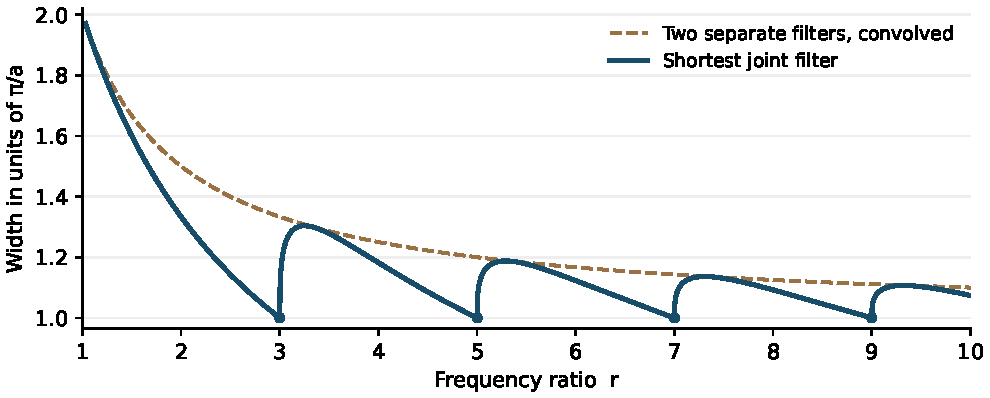
\includegraphics[width=.88\linewidth]{pair_width.pdf}
\caption{Optimal logarithmic width for two frequencies $a$ and $ra$, divided by
$\pi/a$. Odd integer ratios cancel at the single-frequency minimum.
Immediately to their right the increase has order $(r-n)^{1/3}$.}
\end{figure}

\section{The distribution of the optimal width at Dirichlet zeros}
\label{pair:limit-sec}
Fix a positive ordinate $a$ of a nontrivial Dirichlet zero. Fix a
primitive Dirichlet character $\chi$, possibly of conductor one, and let
$b>a$ run through the positive ordinates of its nontrivial zeros,
with multiplicity. The character supplying $a$ can be chosen independently
of $\chi$. Using Dirichlet GRH, let $d(a,b)$ be the minimum support
diameter of a positive probability measure $\mu$ for which
\[
 \int e^{(1/2+ia)t}\,d\mu(t)=\int e^{(1/2+ib)t}\,d\mu(t)=0.
\]
These are the two multipliers that occur when log-dilations are averaged
in a smoothed prime explicit formula. The extra diameter beyond that
needed for $a$ alone, measured in units of $1/b$, is
\[
 E_a(b)=b\bigl(d(a,b)-\pi/a\bigr)
       =r\bigl(D(r)-\pi\bigr),\qquad r=b/a.
\]
The equality uses the common tilt and scaling in Section~\ref{pair:sec}.
The two endpoint-pair convolution gives $0\le E_a(b)\le\pi$.

\begin{theorem}[A universal law for the extra width]\label{pair:limit}
Let $U$ be uniform on $(0,\pi)$. For $0<u<\pi$ define
$Y(u)\in(0,\pi/2)$ and $Z(u)\in(0,\pi-u)$ by
\[
 \tan Y=u+Y,\qquad \sin(u+Z)=Z\cos Y .
\]
Let $N_{\chi,a}(T)$ count the ordinates $a<b\le T$ with multiplicity.
For each continuous real function $f$ on $[0,\pi]$,
\[
 \lim_{T\to\infty}\frac{1}{N_{\chi,a}(T)}
       \sum_{a<b\le T} f(E_a(b))
       =\frac1\pi\int_0^\pi f(2Z(u))\,du .
\]
The law of $2Z(U)$ has no atoms and has support $[0,\pi]$.
In particular $\liminf_{b\to\infty} E_a(b)=0$ and
$\limsup_{b\to\infty} E_a(b)=\pi$ for every fixed choice of $a$ and
$\chi$. Every open subinterval of $[0,\pi]$ receives a positive
limiting fraction of the ordinates.
\end{theorem}
\begin{proof}
By Akbary and Murty \cite[Corollary~8]{AM}, the positive nontrivial zero
ordinates of $L(s,\chi)$ are equidistributed modulo one after
multiplication by any fixed nonzero real constant. Apply this with
$1/(2a)$. Thus the phases
\[
 u_b=\pi\left\{\frac{b}{2a}-\frac12\right\},\qquad
 \{x\}=x-\lfloor x\rfloor ,
\]
are equidistributed on $[0,\pi)$. This fact about ordinates is
unconditional. Dirichlet GRH identifies the same real part $1/2$ for
all the exponential multipliers. In the zeta case the equidistribution
step also follows from Landau's fixed-$x$ formula
\cite{Landau,FSZ}. For $x=\exp(\pi k/a)$ with $k$ a positive integer,
RH gives
\[
 \sum_{0<\gamma\le T} e^{i\pi k\gamma/a}
 =x^{-1/2}\!\sum_{0<\gamma\le T} x^{\rho}=O_{a,k}(T).
\]
Division by $N(T)\sim T\log T/(2\pi)$ proves the Weyl criterion.

Fix $0<\eta<\pi/2$. On the phase interval
$[\eta,\pi-\eta]$, Section~\ref{pair:detune} gives
$E_a(b)=2Z(u_b)+O_\eta((b/a)^{-2})$ uniformly as $b\to\infty$.
By uniform continuity of $f$, averaging their $f$-values over this
interval introduces an error tending to zero. The omitted phases have
limiting proportion $2\eta/\pi$. The profile $Z$ is continuous on the
interior by the implicit equations, so equidistribution on the retained
interval applies to $f(2Z)$. Letting $\eta\downarrow0$ proves the
formula; the same upper bound $2Z\le\pi$ on interior phases follows by
taking $r=n+2u/\pi$ with $n$ an increasing sequence of odd integers.

For the support, $Z(u)\to0$ as $u\uparrow\pi$ by its defining
interval. At $u_* = \arctan(2/\pi)$ the two equations have
$Y=\pi/2-u_*$ and $Z=\pi/2$. Thus continuity and positivity of
Lebesgue measure on open intervals show that the support is all of
$[0,\pi]$. The profile is real analytic in the open phase interval:
the derivative of $\tan Y-Y$ is strictly positive there, and
$\sin(u+z)/z$ has strictly negative derivative at its root
value $\cos Y$. It is nonconstant by the two values just obtained.
Every level set in the interior therefore has Lebesgue measure zero.
The limiting law has no atoms, which permits interval indicators by
continuous approximation and proves the asserted limits.
\end{proof}


\subsection*{How often the optimal width is near either extreme}
Write $X=2Z(U)$ for the limit variable, where $U$ is uniform on $(0,\pi)$.
Two different mechanisms govern its endpoints. Put $t_0=\pi/2$ and
let $Y_\pi\in(0,\pi/2)$ solve $\tan Y_\pi=\pi+Y_\pi$. Then
\begin{equation}\label{eq:edges}
\begin{aligned}
 \Pr(X\le e)&\sim \frac{1+\cos Y_\pi}{2\pi}\,e,\\[2pt]
 \Pr(X\ge\pi-e)&\sim
 \frac{2}{\pi}\frac{\sqrt{2t_0^3}}{1+t_0^2}\,\sqrt{e}
 \qquad(e\downarrow0).
\end{aligned}
\end{equation}
Both are statements about the limiting law. The zero-height limit is
taken first.

\begin{proof}
At $u\downarrow0$, the equation for $Y$ gives
$u=\tan Y-Y\sim Y^3/3$. Substitution of $z=tY$ into
$\sin(u+z)-z\cos Y$, followed by division by $Y^3$, gives
$(2-t)(t+1)^2/6+o(1)$ for fixed $t$. Thus $Z\sim 2(3u)^{1/3}$.
At $u=\pi-v$ the bound $0<Z<v$ gives
$\sin(v-Z)=Z\cos Y$, so $Z\sim v/(1+\cos Y_\pi)$.
Interior intervals have strictly positive minimum. The small-$u$ branch
therefore contributes $O(e^3)$ to the first probability, and the other
branch gives its displayed linear term, by squeezing each sublevel set
between the corresponding endpoint intervals.

For the upper edge write $F(u,z)=\sin(u+z)-z\cos Y(u)$.
Its $z$-derivative is negative at $Z(u)$, and $Y'=\cot^2Y$.
At a stationary point of $Z$, the equations $F=F_u=0$ give
$\cot(u+Z)=-\cot Y$. Hence $u+Z=\pi-Y$ and $Z=\tan Y=u+Y$.
This forces $Z=t_0$ and $u=u_*=\arctan(1/t_0)$.
Conversely these values satisfy both equations, and the positive interior
maximum must occur there. At this point, writing $t=t_0$, we have
\[
 F_z=-2\cos Y,\qquad F_{uu}=-\cos Y\,\frac{(1+t^2)^2}{t^3},
 \qquad Z''(u_*)=-\frac{(1+t^2)^2}{2t^3}.
\]
Indeed $Y'=1/t^2$ and $Y''=-2(1+t^2)/t^5$ there. Taylor expansion
of $2Z$ at its unique maximum shows that the length of the set where
$2Z\ge\pi-e$ is asymptotic to $2\sqrt{e/|Z''(u_*)|}$.
Division by $\pi$ proves the second formula.
\end{proof}
For reference, numerical evaluation gives $\Pr(X\le\pi/2)=0.328039432\ldots$
and a median of $0.711649171\ldots$ for $X/\pi$. These values are computed
by inverting $2Z$ on each side of $u_*$ in \texttt{law\_profile.py}.
The unique stationary point proved above makes both inversions monotone.

\subsection{The arithmetic second term for smooth width statistics}
Let $N_\chi^+(T)$ count the nontrivial zeros of $L(s,\chi)$ with
$0<\gamma\le T$, including multiplicities. Write $\{x\}=x-\lfloor x\rfloor$.
\begin{theorem}[Arithmetic bias]\label{arith:bias}
Fix $a>0$, a primitive Dirichlet character $\chi$ and a smooth real
function $\varphi$ compactly supported in $(0,\pi)$. Put
$\alpha=1/(2a)$ and $H(t)=\varphi(2Z(\pi\{t-1/2\}))$, extended by
zero at the seam. Then
\[
 \sum_{a<\gamma\le T}\varphi(E_a(\gamma))
 =N_\chi^+(T)\int_0^1 H(t)\,dt+
 T\int_0^1 H(t)g_{\chi,\alpha}(t)\,dt+o(T).
\]
The correction density is zero unless
$\alpha=A\log p/(2\pi B)$ for a prime $p$ and relatively prime positive
integers $A,B$. At such an $\alpha$ it is
\[
 g_{\chi,\alpha}(t)=-\frac{\log p}{\pi}\Re
 \sum_{k\ge1}\frac{\chi(p)^{Ak}e^{-2\pi i Bkt}}{p^{Ak/2}}.
\]
In particular a prime dividing the conductor also gives zero correction.
\end{theorem}
\begin{proof}
For $r=\gamma/a$ and the preceding odd integer $n$, the band phase is
$u=\pi(r-n)/2=\pi\{\alpha\gamma-1/2\}$, and
$E_a(\gamma)=r(D(r)-\pi)=2z$ away from the odd ratios.
On compact subintervals of $(0,\pi)$ the expansion after
Theorem~\ref{pair:saturation} gives $2z=2Z(u)+O(r^{-2})$.
Both profiles vanish uniformly at the seam in the following sense.
For $r\to\infty$ and $u\to\pi$ we have $0<z<\pi-u$. For $u\to0$ the
contact equation $\tan y=r\tan((u+y)/r)$ bounds $\tan y$ and forces any
limit to solve $\tan y=y$, so $y\to0$. Then $S/r\to1$ and the endpoint
equation forces every subsequential limit of $z$ to solve $\sin z=z$ on
$[0,\pi]$. Thus $z\to0$. The limiting equations give the same assertions
for $Z$. Exact odd ratios have $E_a=0$. Consequently $H$ is smooth and
periodic, and for all sufficiently large $r$ the two tests vanish on a
fixed neighbourhood of the seam. On its complement their difference
is $O_\varphi(r^{-2})$. The zero count gives
$\sum_{\gamma>a}\gamma^{-2}<\infty$, so the replacement of the test
by $H(\alpha\gamma)$ costs $O(1)$ in the full sum.

Apply Ford, Soundararajan and Zaharescu \cite[Theorem~5, formula (3.2)]{FSZ} to $H$. To check the orientation for complex characters,
the integral of $e^{2\pi i Bkt}g_{\chi,\alpha}(t)$ is
$-(\log p)\chi(p)^{Ak}/(2\pi p^{Ak/2})$ for $k\ge1$.
This agrees with the positive-ordinate Landau formula at
$x=e^{2\pi Bk\alpha}=p^{Ak}$.
\end{proof}


\subsection*{Examples with actual zeta zeros}
For $a=\gamma_1$ the following entries come from the exact optimizer,
using rounded ordinates from the LMFDB tables \cite{LMFDB}. The last
column converts logarithmic width into the ratio of the largest and smallest
arguments of the prime sum. The script \texttt{pair\_examples.py} reproduces
the entries, the tilted masses, and Figure~1.
\begin{center}
\begin{tabular}{rrrrr}
\toprule
Second zero & $\gamma_j/\gamma_1$ & separate widths summed & joint width & dilation ratio\\
\midrule
$j=2$  & 1.487262 & 0.371703420 & 0.357438197 & 1.429662206\\
$j=10$ & 3.521387 & 0.285377967 & 0.283311228 & 1.327518259\\
$j=20$ & 5.457824 & 0.262983914 & 0.262502497 & 1.300179715\\
\bottomrule
\end{tabular}
\end{center}
For the first pair the exact width is $4\pi/(\gamma_1+\gamma_2)$.
In a forward average the three log offsets are $0,d/2,d$, with tilted
weights approximately $0.300320636,\,0.448508965,\,0.251170400$.
The exact weights cancel both modes for every admissible $W$.
Rounded entries illustrate the formula.


\section{Wide arithmetic progressions of frequencies}
\label{sec:progressions}
Fix positive integers $N,b$ and an integer $K\ge0$. On the circle of
circumference one let $M_K=M_K(N,b)$ be the supremum of the lengths of
intervals on which some real trigonometric polynomial with spectrum in
$\{\pm(N+jb):0\le j\le K\}$ is strictly positive. The same supremum
results from asking that the polynomial have no zero there, by continuity
and change of sign. In this section the frequency $m$ denotes $e^{2\pi i m x}$.

\begin{theorem}[Wide-step limit and sharp order]\label{thm:wide}
Suppose $b\ge2N$, write $\beta=N/b$, and put $c=\lceil1/(2\beta)\rceil$.
If $b/(2N)$ is an integer, then $bM_K=c$ for every $K$.
Otherwise for all sufficiently large $K$
\begin{equation}\label{eq:rate}
   \frac{2\beta c-1}{K+2\beta}
       \ \le\ c-bM_K\ \le\ \frac{C_\beta}{K}.
\end{equation}
The left inequality holds for every $K\ge0$. Consequently
$\lim_{K\to\infty}M_K=\lceil b/(2N)\rceil/b$ in both cases.
\end{theorem}

The narrow-step answer of Kozma and Oravecz is $(K+1)/(2N+Kb)$ for $b<2N$
\cite[Theorem 3]{KO}. They ask what happens when $b\ge2N$.
Theorem~\ref{thm:wide} answers their large-$K$ question for every fixed
pair $(N,b)$, and gives the exact finite-$K$ answer at resonance.
Corollary~\ref{pair:gap} gives the exact $K=1$ answer for every pair.
For general nonresonant progressions, an exact formula at every finite $K$ remains open in this analysis.

\begin{proof}
Use the angular coordinate $t=2\pi b x$. The allowed functions are real
parts of $e^{i\beta t}P(e^{it})$, where $P$ has degree at most $K$.
A length of $2\pi$ in $t$ corresponds to $1/b$ on the original circle.

\emph{The bound from a whole progression.}
Write $\theta=2\pi\beta$. At $t=2\pi j$ every prescribed Fourier mode
has value $e^{ij\theta}$. These points for $0\le j\le c$ have zero in their
convex hull. Indeed the consecutive circular gaps are $\theta\le\pi$ and
$2\pi-c\theta\le\pi$, with $c\theta<2\pi$. Thus a probability measure
on these nodes annihilates every frequency in the progression, including
every extension in $K$. Translation moves it into any interval of length
$2\pi c$. Strict positivity there is impossible, whence $bM_K\le c$.
At resonance the lowest cosine by itself attains the supremum $1/(2N)=c/b$.
For a nonresonant progression one may use just the three indices $0,c-1,c$,
with weights proportional to
\[
 \sin\theta,\qquad -\sin(c\theta),\qquad \sin((c-1)\theta).
\]
They are positive, and direct complex addition gives zero.

\emph{The finite-degree obstruction.}
In the nonresonant case $c\ge2$. Consider a closed positive interval of
length $2\pi(c-\varepsilon)$ with $0\le\varepsilon<1$. Since it contains
a whole turn, $P$ has no unit-circle root. The net change of the continuous
argument of $e^{i\beta t}P(e^{it})$ on it has absolute value less than $\pi$.
For an exterior root $w$ of $P$,
\[
 \frac{d}{dt}\arg(e^{it}-w)
 =\frac12+\frac{1-|w|^2}{2|e^{it}-w|^2}<\frac12 .
\]
Its net change over $c$ complete turns is zero. Omitting the complementary
arc of length $2\pi\varepsilon$ thus leaves a change of at least
$-\pi\varepsilon$. For an interior root the derivative is positive, so its
change on the positive interval is nonnegative. Adding the changes gives
$2\pi\beta(c-\varepsilon)-K\pi\varepsilon<\pi$. This proves the left
inequality of \eqref{eq:rate} by passage to the supremum. If the interval
has length at most $2\pi(c-1)$, the same bound follows from
$2\beta(c-1)<1$.

\emph{A polynomial positive on a long interval.}
Let $\alpha=2\beta<1$, $0<\rho<1$ and define
\[
 H_\rho(t)=e^{i\beta t}(1-\rho e^{it})^{-\alpha},\qquad
 P_K(z)=\sum_{j=0}^K a_j\rho^j z^j,\qquad
 a_j=\frac{(\alpha)_j}{j!}.
\]
Use the analytic branch positive at the real point $1-\rho$.
If $\psi_\rho(t)$ is the continuous argument of $H_\rho(t)$ starting at
zero, elementary differentiation yields
\[
 \psi_\rho'(t)=\beta\,\frac{1-\rho^2}{|1-\rho e^{it}|^2}>0,\qquad
 \psi_\rho(t+2\pi)=\psi_\rho(t)+2\pi\beta .
\]
For $0<\delta<\pi$, integration of the Poisson kernel, or the tangent
half-angle identity, gives the following exact angular margin. On the
entire interval $[\delta,2\pi c-\delta]$, after rotation by
$e^{-i\pi c\beta}$, the phase of $H_\rho$ is between
$-\pi/2+m$ and $\pi/2-m$, where
\[
 m=\pi\bigl(\tfrac12-(c-1)\beta\bigr)
     -\alpha\arctan\!\left(\frac{1-\rho}{1+\rho}\cot(\delta/2)\right).
\]
Indeed $\psi_\rho(\delta)=\pi\beta-\alpha\arctan((1-\rho)
\cot(\delta/2)/(1+\rho))$ and
$\psi_\rho(2\pi c-\delta)=2\pi c\beta-\psi_\rho(\delta)$.
The fixed first term in $m$ is strictly positive.

For $|z|=\rho$ the relative truncation error satisfies
\begin{align*}
 \left|(1-z)^\alpha\sum_{j>K}a_jz^j\right|
 &\le 2a_{K+1}\rho^{K+1}|1-z|^{\alpha-1}\\
 &\le 2(K+2)^{\alpha-1}\rho^{K+1}(1-\rho)^{\alpha-1}.
\end{align*}
For the first inequality multiply the tail by $1-z$ and telescope the
decreasing coefficients. For the second use
$a_j=\prod_{\ell=1}^j(1-(1-\alpha)/\ell)\le (j+1)^{\alpha-1}$.
Choose $\rho=1-D/(K+2)$ and $\delta=U/(K+2)$.
The error is at most $2D^{\alpha-1}\exp(-D(K+1)/(K+2))$. First take
$D$ large enough to make this less than half the sine of half of the
fixed angular margin for large $K$. Then take $U/D$ large enough that $m$
exceeds half the fixed margin, using $\cot(\delta/2)\le2/\delta$.
The real part of the rotated, truncated polynomial is now strictly
positive on the indicated interval. It gives
$bM_K\ge c-U/(\pi(K+2))$, as required.
\end{proof}

A numerical certificate can use the same phase margin without sampling
any point of the interval. The script \texttt{progression\_check.py}
bounds the tail, the angle margin, and its sine by rational arithmetic.
Three of its nine enclosures are shown below.
\begin{center}
\begin{tabular}{rrrcc}
\toprule
$N$ & $b$ & $K$ & lower bound for $bM_K$ & upper bound for $bM_K$\\
\midrule
1 & 3 & 64 & 1.97945454 & 1.99484537\\
2 & 5 & 256 & 1.98724292 & 1.99766356\\
2 & 7 & 1024 & 1.99924300 & 1.99986057\\
\bottomrule
\end{tabular}
\end{center}

For any finite set of frequencies the convex-hull proof of
Corollary~\ref{pair:gap} identifies the zero-free supremum with the least
diameter of a probability measure annihilating all the frequencies, in
the same coordinate. Existence at the limiting diameter follows from
weak compactness after centering. Thus the infinite progression has a
shortest annihilator of diameter exactly $c/b$ in circle-length units.
The grid measure above attains it. The finite progression provides the
matching lower bound as $K\to\infty$.


\section{A growing collection of actual Dirichlet zeros}
\label{sec:packets}
Fix integers $N,b\ge1$ with $b\ge 2N$, and a primitive Dirichlet character $\chi$, including the conductor-one case. Write $M_K$ for the maximum-gap supremum on the unit circle for the frequencies $N+bj$, $0\le j\le K$. The zeros used below can be chosen afresh at every height.

\begin{theorem}\label{thm:packets}
Fix $p>1$ and $0<\kappa<1/(2p)$. Suppose $K=K(T)\to\infty$ with
$K\le\kappa\log T/\log\log T$. There is a constant $H_\chi$ such that for all large $T$ one may choose a positive zero ordinate $\gamma_j$ of $L(s,\chi)$ in every interval
$[T(N+bj),T(N+bj)+H_\chi]$. For every such choice let $D_T$ be the minimum logarithmic span of a positive probability average canceling all the selected zero terms. Under Dirichlet GRH,
\[
             \bigl|T D_T-2\pi M_K\bigr|\le K^{-p}.
\]
In particular, if $c=\lceil b/(2N)\rceil>b/(2N)$, then
$2\pi c/b-TD_T\asymp_{N,b} K^{-1}$. One may take $p=2$ for every $\kappa<1/4$.
\end{theorem}

\begin{proof}
The count of positive ordinates up to $X$, with multiplicity, is
$X\log X/(2\pi)+c_\chi X+O_\chi(\log X)$
\cite[(3.1)]{FSZ}, following \cite[(1.6)]{rvM}. Taking differences at $X$ and $X+H_\chi$, the gain from the main term exceeds both endpoint errors for sufficiently large fixed $H_\chi$ and all sufficiently large $X$. This applies simultaneously at every $X=T(N+bj)$.

For a vector $\boldsymbol\lambda$ of positive angular frequencies let $W(\boldsymbol\lambda)$ be the shortest interval supporting a probability measure with $\int e^{i\lambda_j u}\rd\mu(u)=0$ for each $j$. Put $\lambda_j=N+bj$ and $\lambda'_j=\gamma_j/T$. Translation and the common critical-line tilt give $TD_T=W(\boldsymbol\lambda')$.
The finite moment duality gives $W(\boldsymbol\lambda)=2\pi M_K$, uniformly bounded by $2\pi c/b$.

Here is the perturbation estimate with the number of constraints retained. Set $d=K+1$, $m=2d+1$, $\delta=K^{-p}$, and initially take the bounded-width source $\boldsymbol\lambda$ and target $\boldsymbol\lambda'$. An optimal measure on $[0,W]$ exists by compactness. By Carath\'eodory's theorem in $2d$ real moment coordinates we may take it to have at most $m$ atoms, so some atom $v$ has mass at least $1/m$. Convolve with the uniform law on $j\Delta$, $0\le j<m$, where $\Delta=\delta/(m-1)$. The resulting probability has width at most $W+\delta$, still annihilates the source, and has mass at least $m^{-2}$ at each $v+j\Delta$. Its target moments have absolute value at most $(W+\delta)H_\chi/T$ by $|e^{ix}-e^{iy}|\le|x-y|$.

Order the signed target frequencies together with zero as $\xi_0<\cdots<\xi_{m-1}$. Their spacing is bounded below in terms of $N,b$ and their span is $O_{N,b}(d)$. On removing the unit row factors $e^{i\xi_\ell v}$, the matrix for changing the $m$ reserved weights is $V_{\ell j}=z_\ell^j$, $z_\ell=e^{i\xi_\ell\Delta}$. For large $K$, all arguments lie on an arc of length less than $\pi$, so
$|z_\ell-z_h|\ge C\Delta |\ell-h|$ with $C>0$ independent of $K,T$. Each coefficient of the $\ell$th cardinal interpolation polynomial is bounded by
\[
 \frac{2^{2d}}{(C\Delta)^{2d}\ell!(2d-\ell)!}
 \le (C'/\delta)^{2d},
\]
using $\ell!(2d-\ell)!\ge(d!)^2\ge(d/e)^{2d}$. These coefficients are the entries of $V^{-1}$. Solving for corrections to the moments, with zero change at frequency zero, therefore costs at most $O_\chi(m(W+\delta)(C'/\delta)^{2d}/T)$ in each weight. The corrections are real by conjugate symmetry and uniqueness. Their size is at most $T^{-1+2p\kappa+o(1)}<m^{-2}$. Thus the corrected measure is positive of mass one, and $W(\boldsymbol\lambda')\le W(\boldsymbol\lambda)+\delta$. Both widths are now uniformly bounded. Interchanging the source and target gives the reverse inequality with the same $\delta$. The nonresonant conclusion follows from the sharp finite-degree gap estimate since $K^{-p}=o(K^{-1})$.
\end{proof}

\section{Further questions}
The two-frequency cost depends only on a single ratio. Three arbitrary
ordinates give a moment curve in six real dimensions. An explicit classification
of its supporting polynomials would extend the prime-sum result to triples.
For the wide-step progression theorem, the order $1/K$ of the deficit is
sharp. Does $K(c-bM_K)$ converge, and which polynomials attain the leading
constant? Finally, a quantitative rate in the zero-ordinate distribution
law would require discrepancy estimates that can resolve the neighborhood of
the maximum of its phase profile. This last issue affects how quickly finite
lists of zeros approximate the limiting upper tail.

\begin{thebibliography}{99}
\bibitem{Article} ProveIt Contributors. \emph{Beyond the Riemann hypothesis
for Dirichlet $L$-functions: consequences, transfers and limits}. 26 November
2026, especially \texttt{sections/rec.tex}, subsection on shortest positive
dilation averages. \href{\baseurl/tree/b6253012cf30c80a989c871906e097a27f23a27c/Analysis/GeneralizedRiemannHypothesis/Article}{Pinned article}.
\bibitem{Nearby} \emph{Positive averaging with logarithmic support at Dirichlet
zeros}. ProveIt research note, 26 November 2026.
\href{\baseurl/tree/b6253012cf30c80a989c871906e097a27f23a27c/Analysis/GeneralizedRiemannHypothesis/Research/logarithmic_dirichlet_zero_filters_2026-11-26}{Pinned report}.
\bibitem{Vendor} \texttt{lsernau/grh-lean}. Readable edition, upstream
commit \texttt{72fead102f66}.
\href{\baseurl/tree/b6253012cf30c80a989c871906e097a27f23a27c/Analysis/GeneralizedRiemannHypothesis/vendor/grh-lean}{Pinned vendor directory}.
\bibitem{KO} G. Kozma and F. Oravecz. On the gaps between zeros of
trigonometric polynomials. \emph{Real Analysis Exchange} \textbf{28}
(2002/03), 447--454. Theorems 2--3 and Question 1.
\href{https://arxiv.org/abs/math/0601021}{Authors' preprint}.
\bibitem{FSZ} K. Ford, K. Soundararajan and A. Zaharescu.
On the distribution of imaginary parts of zeros of the Riemann zeta function, II.
\emph{Mathematische Annalen} \textbf{343} (2009), 487--505,
especially \S3, Lemma 2.
\href{https://arxiv.org/abs/0805.2745}{Authors' preprint}.
\bibitem{AM} A. Akbary and M. R. Murty. Uniform distribution of zeros of
Dirichlet series. \emph{CRM Proceedings and Lecture Notes} \textbf{46}
(2008), 143--158. \href{https://doi.org/10.1090/crmp/046/10}{DOI}.
\bibitem{rvM} A. Selberg. Old and new conjectures and results about a class
of Dirichlet series. \emph{Proceedings of the Amalfi Conference on Analytic
Number Theory} (Maiori, 1989), University of Salerno, 1992, 367--385.
\bibitem{Landau} E. Landau. \"Uber die Nullstellen der $\zeta$-Funktion.
\emph{Mathematische Annalen} \textbf{71} (1911), 548--568.
\bibitem{Crain} E. A. Crain, W. E. Singhose and W. P. Seering. Derivation and properties
of convolved and simultaneous two-mode input shapers. \emph{IFAC Proceedings
Volumes} (1996). \href{https://doi.org/10.1016/S1474-6670(17)58856-4}{DOI}.
\bibitem{Rappole} B. W. Rappole, N. C. Singer and W. P. Seering.
Multiple-mode impulse shaping sequences for reducing residual vibrations.
\emph{Machine Elements and Machine Dynamics}, ASME, \textbf{71} (1994), 11--16.
\href{https://web.mit.edu/shaping/www/dates.html}{MIT publication list}.
\bibitem{LMFDB} The LMFDB Collaboration. \emph{Zeros of $\zeta(s)$},
tabulated positive ordinates. \url{https://www.lmfdb.org/zeros/zeta/}.
\end{thebibliography}
\end{document}
